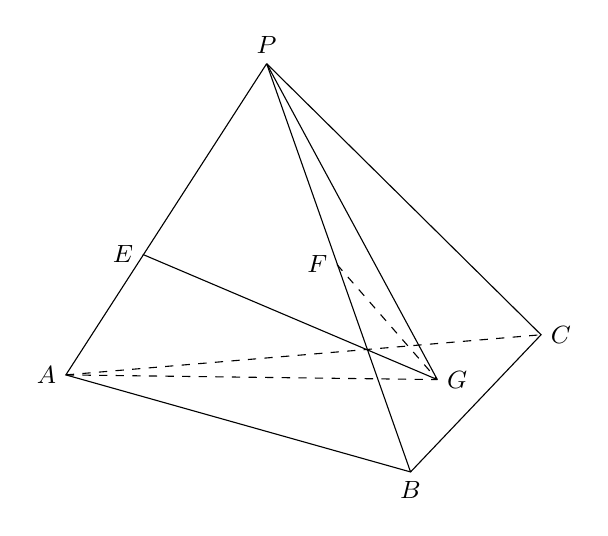
\begin{tikzpicture}[scale=.85, every node/.style={font=\small}]
  \coordinate (P) at (3.0,6.1);
  \coordinate (A) at (0,1.45);
  \coordinate (B) at (5.15,0);
  \coordinate (C) at (7.1,2.05);
  \coordinate (E) at (1.15,3.25);
  \coordinate (F) at (4.05,3.1);
  \coordinate (G) at (5.55,1.38);
  \draw (P)--(A)--(B)--(C)--(P) (P)--(B);
  \draw (E)--(G) (P)--(G);
  \draw[dashed] (A)--(C) (A)--(G) (F)--(G);
  \node[above] at (P) {$P$};
  \node[left] at (A) {$A$};
  \node[below] at (B) {$B$};
  \node[right] at (C) {$C$};
  \node[left] at (E) {$E$};
  \node[left] at (F) {$F$};
  \node[right] at (G) {$G$};
\end{tikzpicture}
